%% Unit 3: Process of Product Design
%% Included from main.tex via %% Unit 3: Process of Product Design
%% Included from main.tex via %% Unit 3: Process of Product Design
%% Included from main.tex via %% Unit 3: Process of Product Design
%% Included from main.tex via \include{./units/unit3}
%% Requires the macros/colours defined in main.tex's preamble.

%==============================================================================
\section{Process of Product Design}
%==============================================================================
\unitdivider{III}{Process of Product Design}{Engineering design, prototyping \& testing}

\begin{frame}{Engineering Product-Design Process}
  \bigfig{product_design_process.png}{A structured flow from identifying a need to manufacture \& launch.}
\end{frame}

\begin{frame}{Design-Thinking Approach to Product Design}
  \accentrule\\[0.3em]
  \begin{columns}[T]
    \begin{column}{0.5\textwidth}\small
      \textbf{Traditional engineering}
      \begin{itemize}\small
        \item Requirements defined up front.
        \item Linear, specification-driven.
        \item User feedback comes late.
      \end{itemize}
    \end{column}
    \begin{column}{0.5\textwidth}\small
      \textbf{Design-thinking infused}
      \begin{itemize}\small
        \item \kwt{User needs} continuously explored.
        \item \kwt{Iterative} — prototype \& test early.
        \item Feedback loops at \emph{every} stage.
      \end{itemize}
    \end{column}
  \end{columns}
  \vspace{0.3em}
  \begin{block}{Best in class}\scriptsize
    Great products (e.g.\ intuitive smartphones, ergonomic tools,
    well-designed appliances) combine \emph{function}, \emph{form} and
    \emph{delight} — form follows function \emph{and} feeling.
  \end{block}
\end{frame}

\begin{frame}{What is a Prototype?}
  \accentrule\\[0.3em]
  \begin{columns}[T]
    \begin{column}{0.52\textwidth}\small
      A \kw{prototype} is an early, testable model of a product used to
      \emph{explore ideas} and \emph{learn} before committing to production.
      \vspace{0.3em}
      \textbf{Why prototype?}
      \begin{itemize}\small
        \item Make ideas \kwt{tangible}.
        \item Test assumptions cheaply.
        \item Communicate with stakeholders.
        \item Fail fast, improve faster.
      \end{itemize}
    \end{column}
    \begin{column}{0.48\textwidth}\small
      \textbf{Types of prototype}
      \begin{itemize}\small
        \item \emph{Low-fidelity} — sketches, paper, cardboard.
        \item \emph{Mid-fidelity} — wireframes, models.
        \item \emph{High-fidelity} — 3-D printed, functional.
      \end{itemize}
    \end{column}
  \end{columns}
\end{frame}

\begin{frame}{Prototype Fidelity Ladder}
  \begin{columns}[c]
    \begin{column}{0.6\textwidth}
      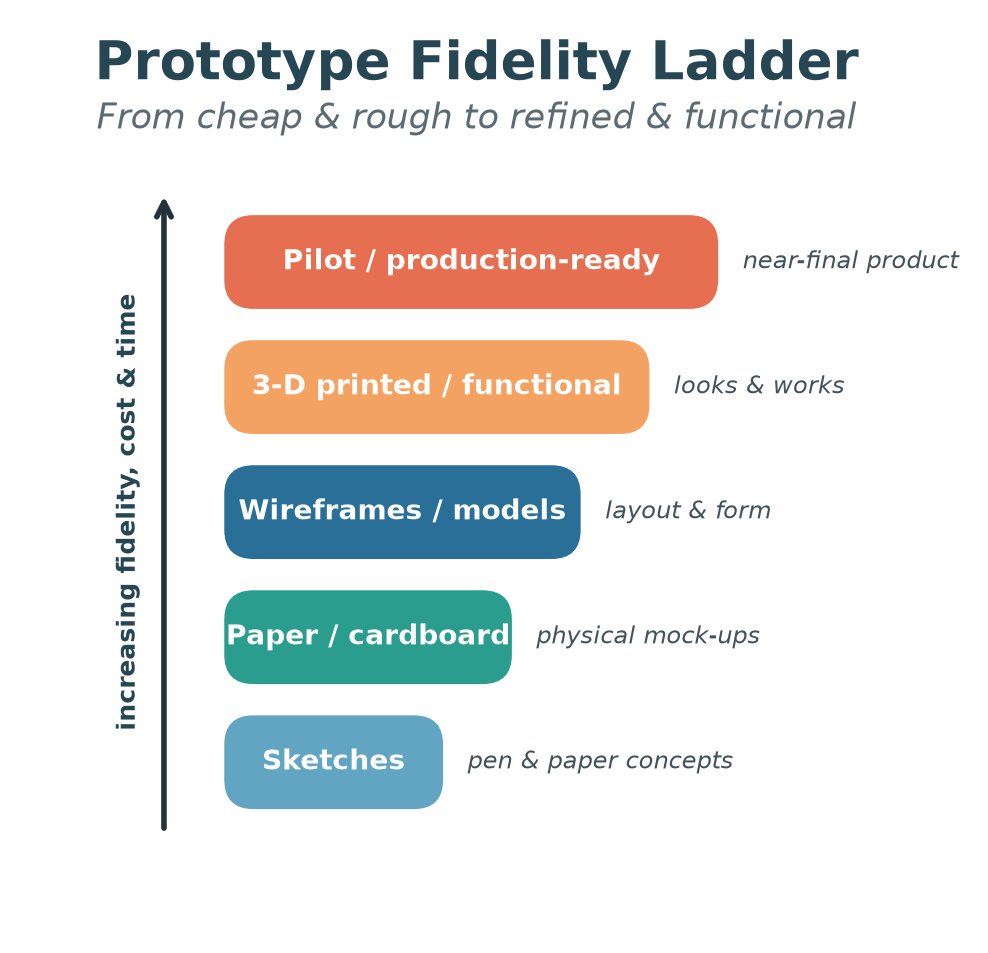
\includegraphics[width=\linewidth]{figures/prototype_fidelity.png}
    \end{column}
    \begin{column}{0.4\textwidth}\scriptsize
      Start \kwt{low} and cheap, climb only as questions demand.
      \vspace{0.3em}
      \begin{itemize}\scriptsize
        \item Low fidelity answers \emph{"is this the right idea?"}
        \item High fidelity answers \emph{"does it work \& feel right?"}
      \end{itemize}
      \vspace{0.3em}
      Each rung costs more time and money — so \emph{learn cheaply first}.
    \end{column}
  \end{columns}
\end{frame}

\begin{frame}{Rapid Prototype Development}
  \begin{columns}[c]
    \begin{column}{0.55\textwidth}
      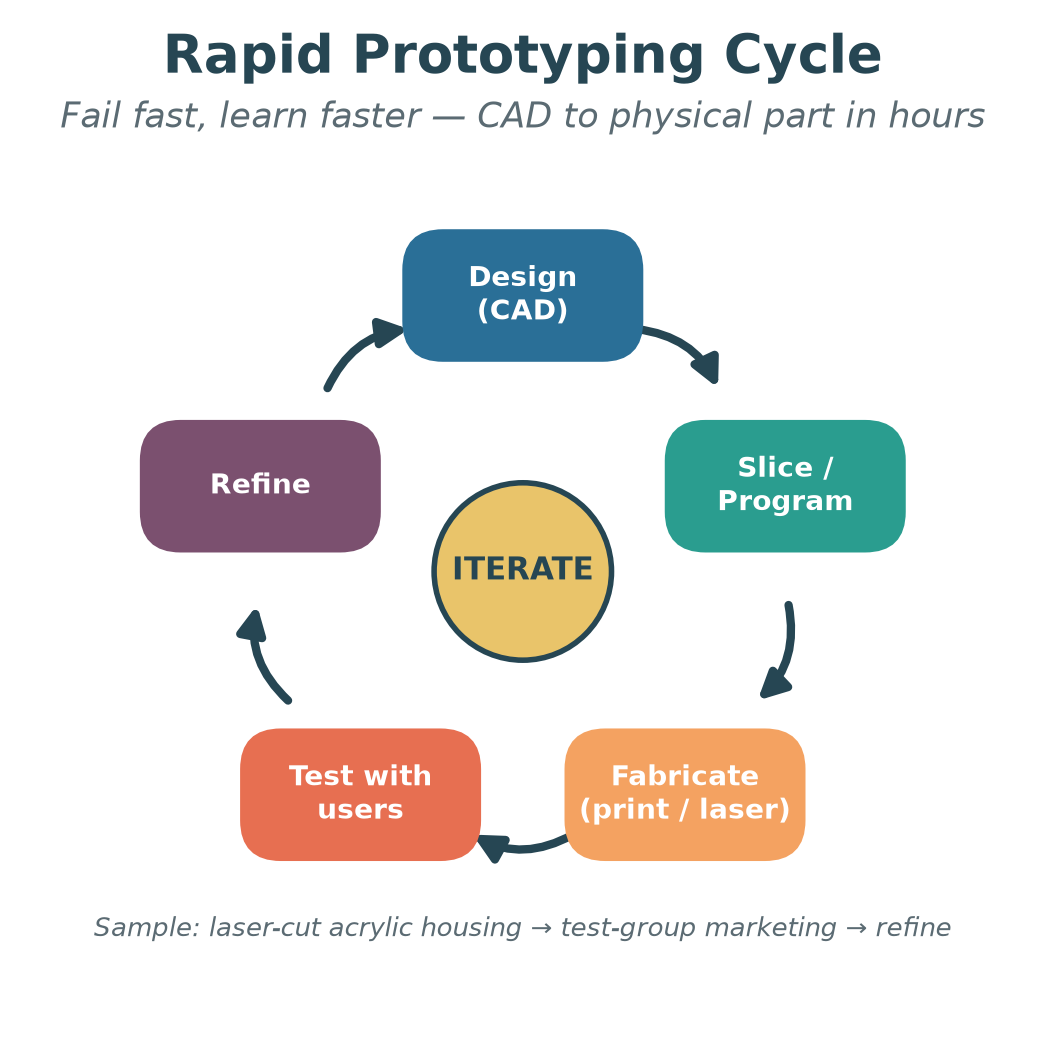
\includegraphics[width=\linewidth]{figures/rapid_prototyping.png}
    \end{column}
    \begin{column}{0.45\textwidth}\scriptsize
      \kw{Rapid prototyping} uses digital fabrication (3-D printing, laser
      cutting, CNC) to go from \kwt{CAD} to a physical part in \emph{hours}.
      \vspace{0.3em}
      \textbf{Testing \& sample marketing}
      \begin{itemize}\scriptsize
        \item Test the prototype with a small \kwt{test group}.
        \item Gather reactions before scaling up.
        \item Refine, then repeat the loop.
      \end{itemize}
    \end{column}
  \end{columns}
\end{frame}

%% Requires the macros/colours defined in main.tex's preamble.

%==============================================================================
\section{Process of Product Design}
%==============================================================================
\unitdivider{III}{Process of Product Design}{Engineering design, prototyping \& testing}

\begin{frame}{Engineering Product-Design Process}
  \bigfig{product_design_process.png}{A structured flow from identifying a need to manufacture \& launch.}
\end{frame}

\begin{frame}{Design-Thinking Approach to Product Design}
  \accentrule\\[0.3em]
  \begin{columns}[T]
    \begin{column}{0.5\textwidth}\small
      \textbf{Traditional engineering}
      \begin{itemize}\small
        \item Requirements defined up front.
        \item Linear, specification-driven.
        \item User feedback comes late.
      \end{itemize}
    \end{column}
    \begin{column}{0.5\textwidth}\small
      \textbf{Design-thinking infused}
      \begin{itemize}\small
        \item \kwt{User needs} continuously explored.
        \item \kwt{Iterative} — prototype \& test early.
        \item Feedback loops at \emph{every} stage.
      \end{itemize}
    \end{column}
  \end{columns}
  \vspace{0.3em}
  \begin{block}{Best in class}\scriptsize
    Great products (e.g.\ intuitive smartphones, ergonomic tools,
    well-designed appliances) combine \emph{function}, \emph{form} and
    \emph{delight} — form follows function \emph{and} feeling.
  \end{block}
\end{frame}

\begin{frame}{What is a Prototype?}
  \accentrule\\[0.3em]
  \begin{columns}[T]
    \begin{column}{0.52\textwidth}\small
      A \kw{prototype} is an early, testable model of a product used to
      \emph{explore ideas} and \emph{learn} before committing to production.
      \vspace{0.3em}
      \textbf{Why prototype?}
      \begin{itemize}\small
        \item Make ideas \kwt{tangible}.
        \item Test assumptions cheaply.
        \item Communicate with stakeholders.
        \item Fail fast, improve faster.
      \end{itemize}
    \end{column}
    \begin{column}{0.48\textwidth}\small
      \textbf{Types of prototype}
      \begin{itemize}\small
        \item \emph{Low-fidelity} — sketches, paper, cardboard.
        \item \emph{Mid-fidelity} — wireframes, models.
        \item \emph{High-fidelity} — 3-D printed, functional.
      \end{itemize}
    \end{column}
  \end{columns}
\end{frame}

\begin{frame}{Prototype Fidelity Ladder}
  \begin{columns}[c]
    \begin{column}{0.6\textwidth}
      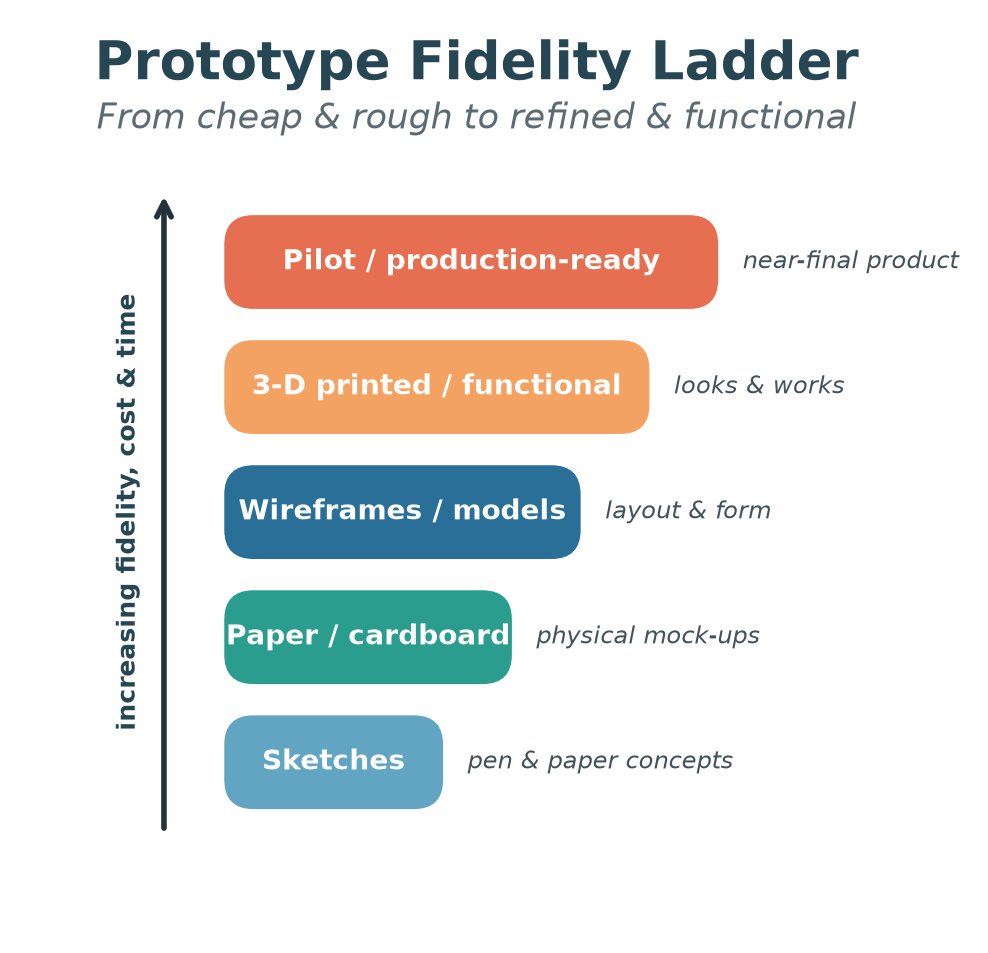
\includegraphics[width=\linewidth]{figures/prototype_fidelity.png}
    \end{column}
    \begin{column}{0.4\textwidth}\scriptsize
      Start \kwt{low} and cheap, climb only as questions demand.
      \vspace{0.3em}
      \begin{itemize}\scriptsize
        \item Low fidelity answers \emph{"is this the right idea?"}
        \item High fidelity answers \emph{"does it work \& feel right?"}
      \end{itemize}
      \vspace{0.3em}
      Each rung costs more time and money — so \emph{learn cheaply first}.
    \end{column}
  \end{columns}
\end{frame}

\begin{frame}{Rapid Prototype Development}
  \begin{columns}[c]
    \begin{column}{0.55\textwidth}
      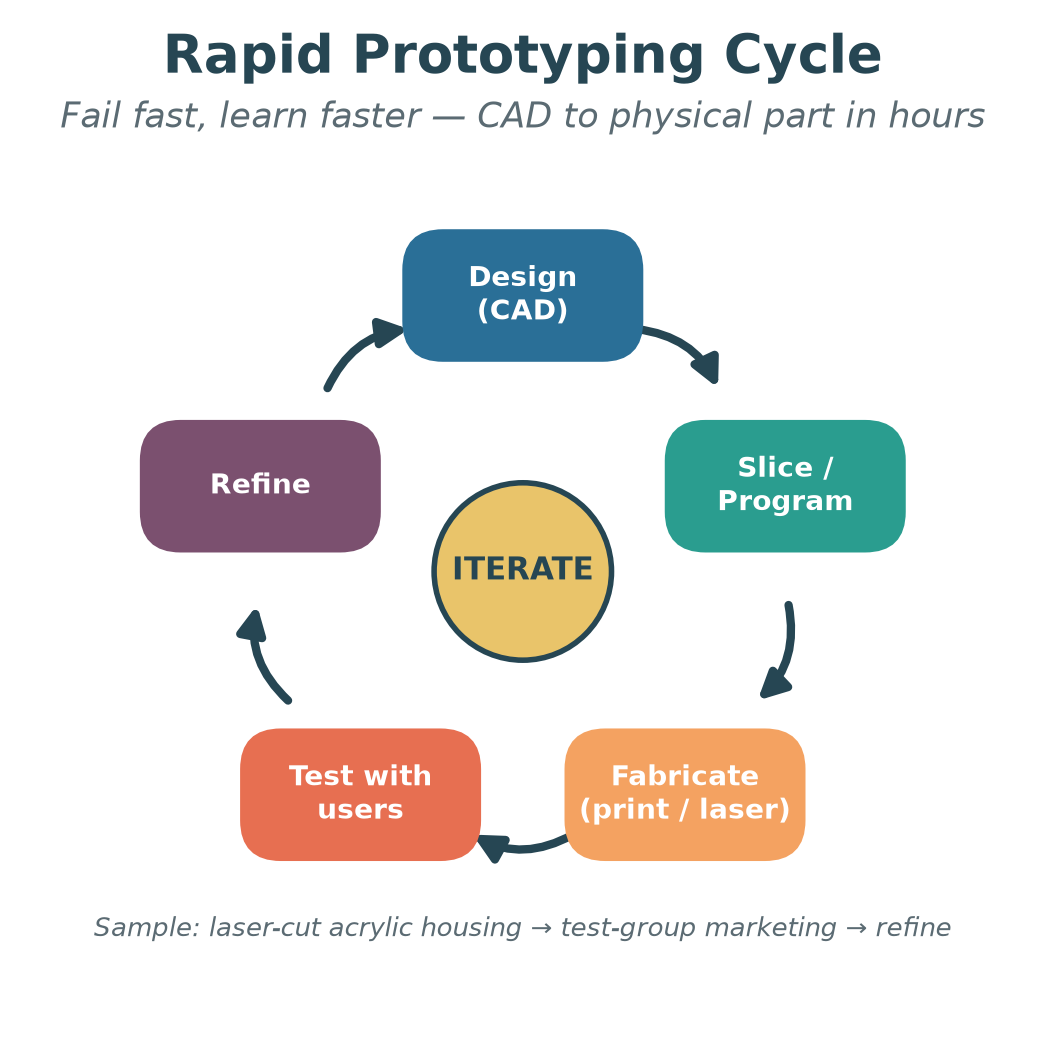
\includegraphics[width=\linewidth]{figures/rapid_prototyping.png}
    \end{column}
    \begin{column}{0.45\textwidth}\scriptsize
      \kw{Rapid prototyping} uses digital fabrication (3-D printing, laser
      cutting, CNC) to go from \kwt{CAD} to a physical part in \emph{hours}.
      \vspace{0.3em}
      \textbf{Testing \& sample marketing}
      \begin{itemize}\scriptsize
        \item Test the prototype with a small \kwt{test group}.
        \item Gather reactions before scaling up.
        \item Refine, then repeat the loop.
      \end{itemize}
    \end{column}
  \end{columns}
\end{frame}

%% Requires the macros/colours defined in main.tex's preamble.

%==============================================================================
\section{Process of Product Design}
%==============================================================================
\unitdivider{III}{Process of Product Design}{Engineering design, prototyping \& testing}

\begin{frame}{Engineering Product-Design Process}
  \bigfig{product_design_process.png}{A structured flow from identifying a need to manufacture \& launch.}
\end{frame}

\begin{frame}{Design-Thinking Approach to Product Design}
  \accentrule\\[0.3em]
  \begin{columns}[T]
    \begin{column}{0.5\textwidth}\small
      \textbf{Traditional engineering}
      \begin{itemize}\small
        \item Requirements defined up front.
        \item Linear, specification-driven.
        \item User feedback comes late.
      \end{itemize}
    \end{column}
    \begin{column}{0.5\textwidth}\small
      \textbf{Design-thinking infused}
      \begin{itemize}\small
        \item \kwt{User needs} continuously explored.
        \item \kwt{Iterative} — prototype \& test early.
        \item Feedback loops at \emph{every} stage.
      \end{itemize}
    \end{column}
  \end{columns}
  \vspace{0.3em}
  \begin{block}{Best in class}\scriptsize
    Great products (e.g.\ intuitive smartphones, ergonomic tools,
    well-designed appliances) combine \emph{function}, \emph{form} and
    \emph{delight} — form follows function \emph{and} feeling.
  \end{block}
\end{frame}

\begin{frame}{What is a Prototype?}
  \accentrule\\[0.3em]
  \begin{columns}[T]
    \begin{column}{0.52\textwidth}\small
      A \kw{prototype} is an early, testable model of a product used to
      \emph{explore ideas} and \emph{learn} before committing to production.
      \vspace{0.3em}
      \textbf{Why prototype?}
      \begin{itemize}\small
        \item Make ideas \kwt{tangible}.
        \item Test assumptions cheaply.
        \item Communicate with stakeholders.
        \item Fail fast, improve faster.
      \end{itemize}
    \end{column}
    \begin{column}{0.48\textwidth}\small
      \textbf{Types of prototype}
      \begin{itemize}\small
        \item \emph{Low-fidelity} — sketches, paper, cardboard.
        \item \emph{Mid-fidelity} — wireframes, models.
        \item \emph{High-fidelity} — 3-D printed, functional.
      \end{itemize}
    \end{column}
  \end{columns}
\end{frame}

\begin{frame}{Prototype Fidelity Ladder}
  \begin{columns}[c]
    \begin{column}{0.6\textwidth}
      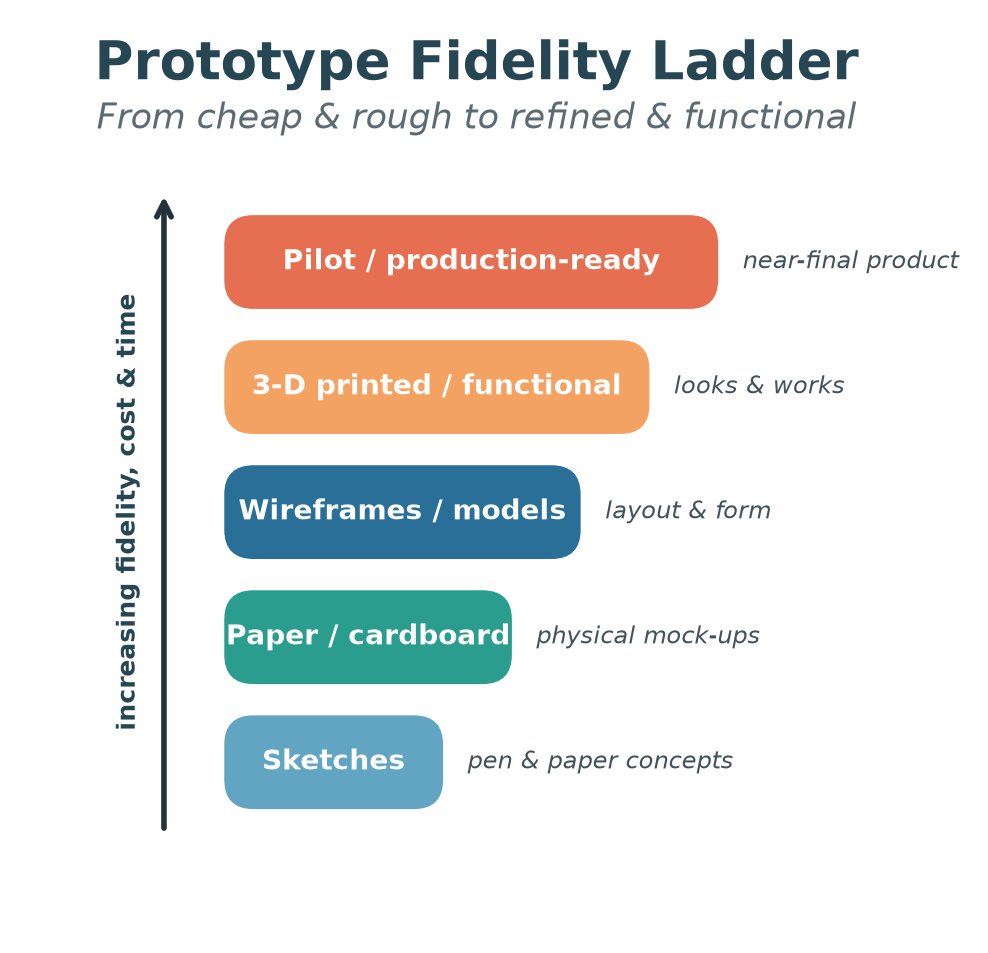
\includegraphics[width=\linewidth]{figures/prototype_fidelity.png}
    \end{column}
    \begin{column}{0.4\textwidth}\scriptsize
      Start \kwt{low} and cheap, climb only as questions demand.
      \vspace{0.3em}
      \begin{itemize}\scriptsize
        \item Low fidelity answers \emph{"is this the right idea?"}
        \item High fidelity answers \emph{"does it work \& feel right?"}
      \end{itemize}
      \vspace{0.3em}
      Each rung costs more time and money — so \emph{learn cheaply first}.
    \end{column}
  \end{columns}
\end{frame}

\begin{frame}{Rapid Prototype Development}
  \begin{columns}[c]
    \begin{column}{0.55\textwidth}
      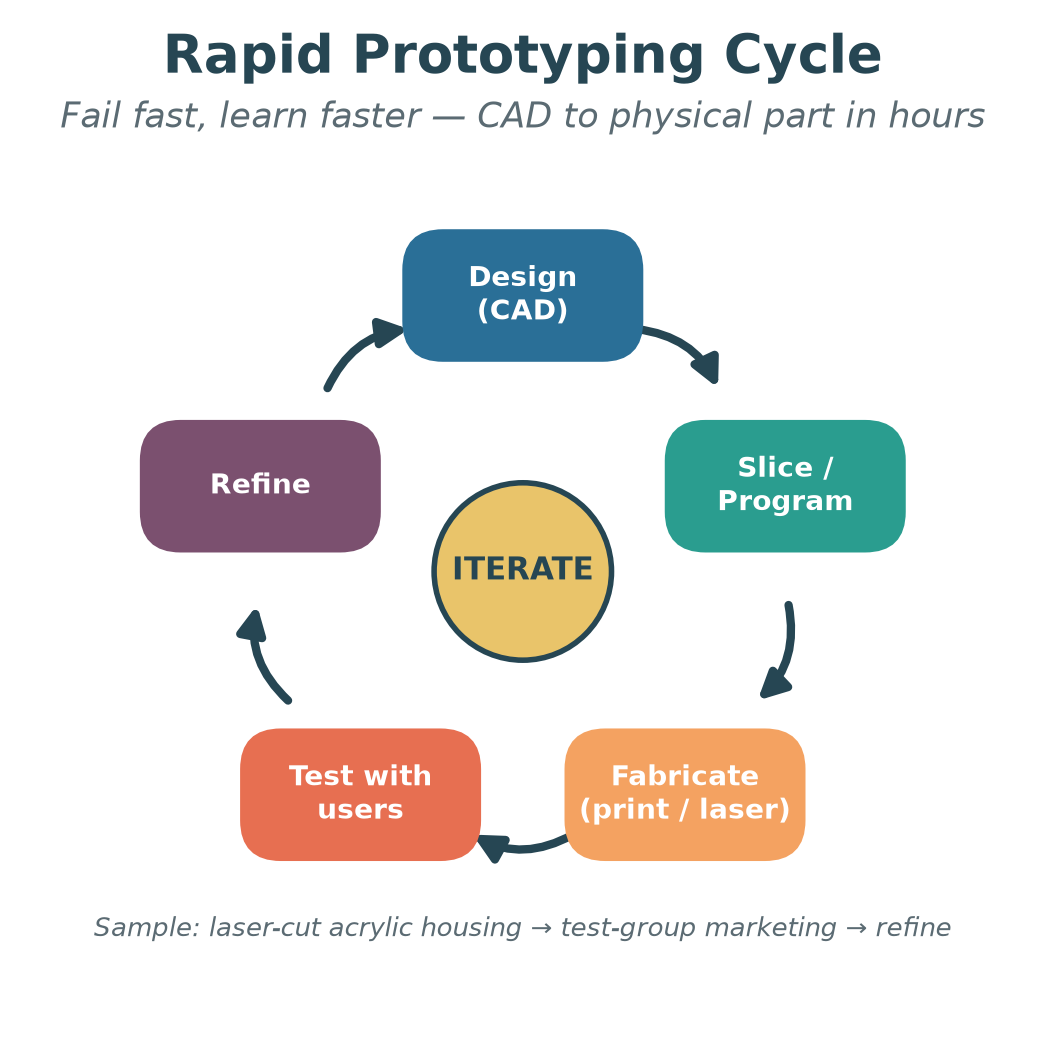
\includegraphics[width=\linewidth]{figures/rapid_prototyping.png}
    \end{column}
    \begin{column}{0.45\textwidth}\scriptsize
      \kw{Rapid prototyping} uses digital fabrication (3-D printing, laser
      cutting, CNC) to go from \kwt{CAD} to a physical part in \emph{hours}.
      \vspace{0.3em}
      \textbf{Testing \& sample marketing}
      \begin{itemize}\scriptsize
        \item Test the prototype with a small \kwt{test group}.
        \item Gather reactions before scaling up.
        \item Refine, then repeat the loop.
      \end{itemize}
    \end{column}
  \end{columns}
\end{frame}

%% Requires the macros/colours defined in main.tex's preamble.

%==============================================================================
\section{Process of Product Design}
%==============================================================================
\unitdivider{III}{Process of Product Design}{Engineering design, prototyping \& testing}

\begin{frame}{Engineering Product-Design Process}
  \bigfig{product_design_process.png}{A structured flow from identifying a need to manufacture \& launch.}
\end{frame}

\begin{frame}{Design-Thinking Approach to Product Design}
  \accentrule\\[0.3em]
  \begin{columns}[T]
    \begin{column}{0.5\textwidth}\small
      \textbf{Traditional engineering}
      \begin{itemize}\small
        \item Requirements defined up front.
        \item Linear, specification-driven.
        \item User feedback comes late.
      \end{itemize}
    \end{column}
    \begin{column}{0.5\textwidth}\small
      \textbf{Design-thinking infused}
      \begin{itemize}\small
        \item \kwt{User needs} continuously explored.
        \item \kwt{Iterative} — prototype \& test early.
        \item Feedback loops at \emph{every} stage.
      \end{itemize}
    \end{column}
  \end{columns}
  \vspace{0.3em}
  \begin{block}{Best in class}\scriptsize
    Great products (e.g.\ intuitive smartphones, ergonomic tools,
    well-designed appliances) combine \emph{function}, \emph{form} and
    \emph{delight} — form follows function \emph{and} feeling.
  \end{block}
\end{frame}

\begin{frame}{What is a Prototype?}
  \accentrule\\[0.3em]
  \begin{columns}[T]
    \begin{column}{0.52\textwidth}\small
      A \kw{prototype} is an early, testable model of a product used to
      \emph{explore ideas} and \emph{learn} before committing to production.
      \vspace{0.3em}
      \textbf{Why prototype?}
      \begin{itemize}\small
        \item Make ideas \kwt{tangible}.
        \item Test assumptions cheaply.
        \item Communicate with stakeholders.
        \item Fail fast, improve faster.
      \end{itemize}
    \end{column}
    \begin{column}{0.48\textwidth}\small
      \textbf{Types of prototype}
      \begin{itemize}\small
        \item \emph{Low-fidelity} — sketches, paper, cardboard.
        \item \emph{Mid-fidelity} — wireframes, models.
        \item \emph{High-fidelity} — 3-D printed, functional.
      \end{itemize}
    \end{column}
  \end{columns}
\end{frame}

\begin{frame}{Prototype Fidelity Ladder}
  \begin{columns}[c]
    \begin{column}{0.6\textwidth}
      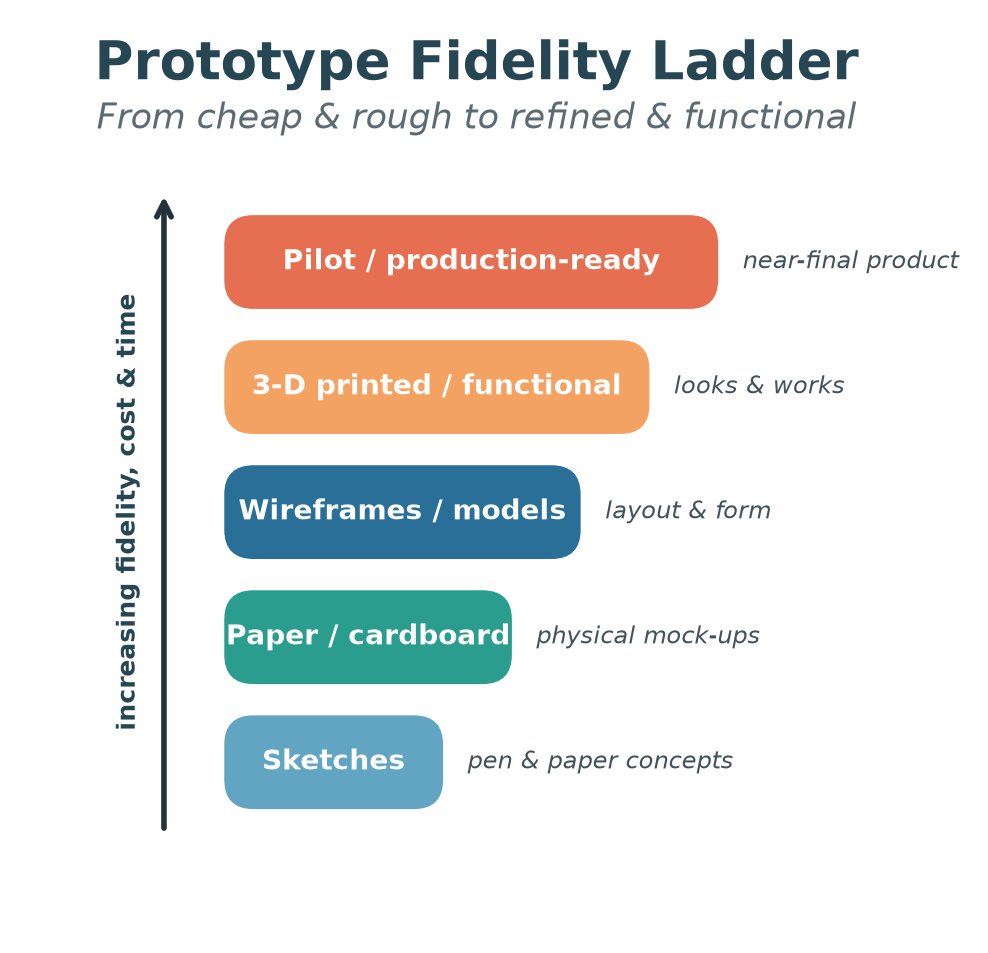
\includegraphics[width=\linewidth]{figures/prototype_fidelity.png}
    \end{column}
    \begin{column}{0.4\textwidth}\scriptsize
      Start \kwt{low} and cheap, climb only as questions demand.
      \vspace{0.3em}
      \begin{itemize}\scriptsize
        \item Low fidelity answers \emph{"is this the right idea?"}
        \item High fidelity answers \emph{"does it work \& feel right?"}
      \end{itemize}
      \vspace{0.3em}
      Each rung costs more time and money — so \emph{learn cheaply first}.
    \end{column}
  \end{columns}
\end{frame}

\begin{frame}{Rapid Prototype Development}
  \begin{columns}[c]
    \begin{column}{0.55\textwidth}
      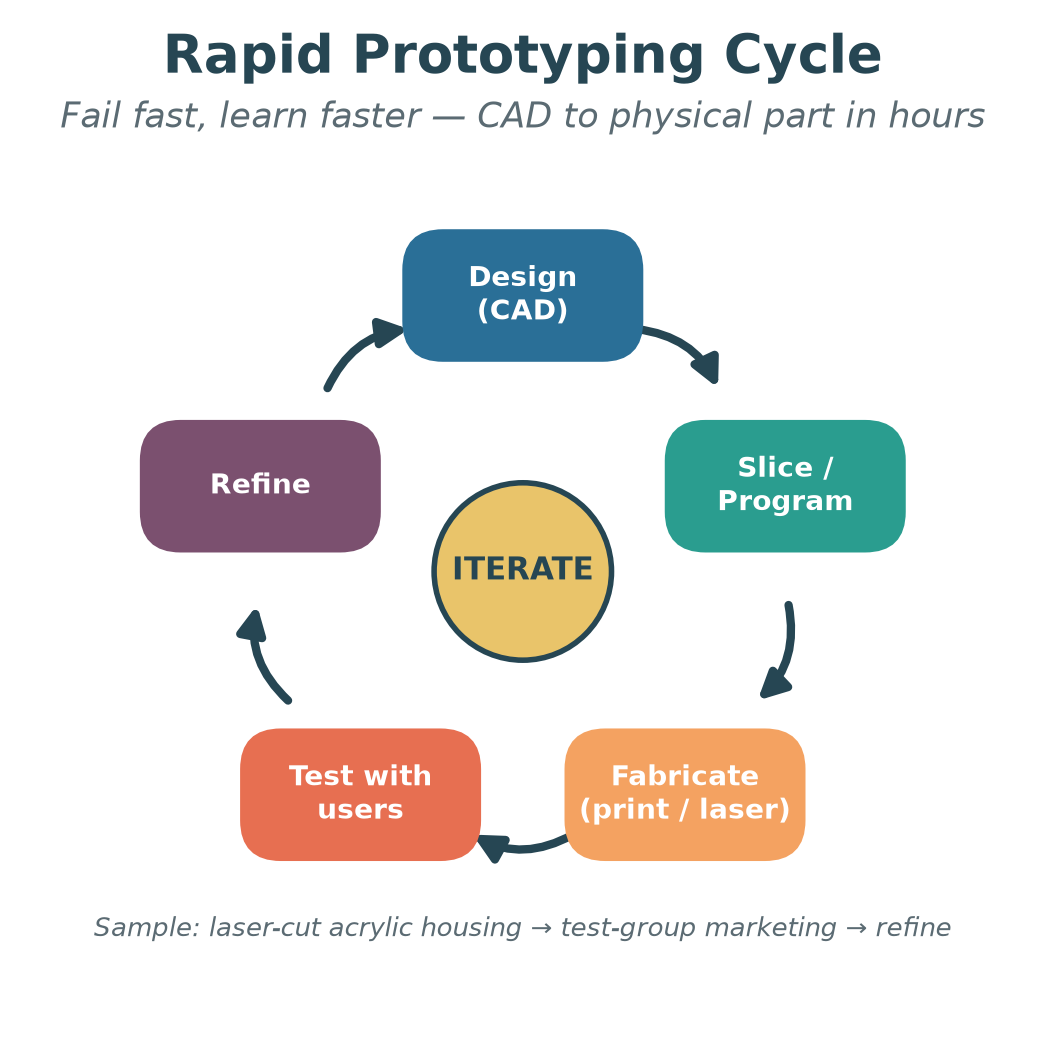
\includegraphics[width=\linewidth]{figures/rapid_prototyping.png}
    \end{column}
    \begin{column}{0.45\textwidth}\scriptsize
      \kw{Rapid prototyping} uses digital fabrication (3-D printing, laser
      cutting, CNC) to go from \kwt{CAD} to a physical part in \emph{hours}.
      \vspace{0.3em}
      \textbf{Testing \& sample marketing}
      \begin{itemize}\scriptsize
        \item Test the prototype with a small \kwt{test group}.
        \item Gather reactions before scaling up.
        \item Refine, then repeat the loop.
      \end{itemize}
    \end{column}
  \end{columns}
\end{frame}
